
%(BEGIN_QUESTION)
% Copyright 2007, Tony R. Kuphaldt, released under the Creative Commons Attribution License (v 1.0)
% This means you may do almost anything with this work of mine, so long as you give me proper credit

Graph just the integral response of a {\it proportional+integral} controller with a proportional band of 75\% and an integral constant of 2 minutes per repeat to the following input conditions.  Assume a control action that is {\it direct-acting}:

$$\includegraphics[width=15.5cm]{i01606x01.eps}$$

The time scale on the chart is minutes:seconds, and the PI algorithm is as follows:

$$m = K_p \left( e + {1 \over \tau_i} \int e \> dt \right) + b$$

\noindent
Where,

$m$ = Controller output (manipulated variable)

$K_p$ = Gain

$e$ = Error signal (PV$-$SP)

$\tau_i$ = Integral time constant

$b$ = Bias

\vskip 10pt

\underbar{file i01606}
%(END_QUESTION)





%(BEGIN_ANSWER)

$$\includegraphics[width=15.5cm]{i01606x02.eps}$$

First, let's convert the given tuning constants into direct-indicating units (gain instead of P.B., and rep/min instead of min/rep):
 
\vskip 10pt

Proportional band = 75\% ; Gain = 1.333
 
\vskip 10pt

2 minutes per repeat = 0.5 repeats per minute
 
\vskip 10pt

\noindent
Now, calculating the accumulated area under each deviation period:
 
\vskip 10pt

Integral action = $K_p {1\over \tau_i} \int e \> dt$
 
\vskip 10pt

Integral action = (gain)(repeats/min)(error-time product)
 
\vskip 10pt

Integral action = (1.333)(0.5/min)(10\%-min)
 
\vskip 10pt

Integral action = 6.667\%
 
\vskip 10pt

\noindent
{\it Output goes from 70\% to 63.33\%}
 
$$\includegraphics[width=15.5cm]{i01606x03.eps}$$

\filbreak

Integral action = $K_p {1\over \tau_i} \int e \> dt$
 
\vskip 10pt

Integral action = (gain)(repeats/min)(error-time product)
 
\vskip 10pt

Integral action = (1.333)(0.5/min)(5\%-min)

\vskip 10pt

Integral action = 3.333\%

\vskip 10pt

\noindent
{\it Output goes from 63.33\% to 60\%}

$$\includegraphics[width=15.5cm]{i01606x04.eps}$$

\filbreak

Integral action = $K_p {1\over \tau_i} \int e \> dt$
 
\vskip 10pt

Integral action = (gain)(repeats/min)(error-time product)
 
\vskip 10pt

Integral action = (1.333)(0.5/min)(3.125\%-min)
 
\vskip 10pt

Integral action = 2.083\%
 
\vskip 10pt

\noindent
{\it Output goes from 60\% to 62.083\%}

$$\includegraphics[width=15.5cm]{i01606x05.eps}$$

\filbreak

Integral action = $K_p {1\over \tau_i} \int e \> dt$
 
\vskip 10pt

Integral action = (gain)(repeats/min)(error-time product)
 
\vskip 10pt

Integral action = (1.333)(0.5/min)(6.25\%-min)
 
\vskip 10pt

Integral action = 4.167\%

\vskip 10pt

\noindent
{\it Output goes from 62.083\% to 66.25\%}

$$\includegraphics[width=15.5cm]{i01606x06.eps}$$

%(END_ANSWER)





%(BEGIN_NOTES)

%INDEX% Control, proportional + integral: graphing controller response

%(END_NOTES)


